\section{物体的浮沉条件}\label{sec:6-3}

既然物体在液体中都受到浮力,那么为什么木块能浮在水面上,而铁块在水里却下沉呢?
钢板在水里会下沉,而用钢板制成的轮船和舰艇却能浮在水面上呢?

要回答上面这些问题,需要全面考虑浸在水里的物体受到的力。
浸在水里的物体受到两个力的作用:
一个是水对物体的向上的浮力,它的大小等于物体排开的水重;
另一个是物体受到的向下的重力(图 \ref{fig:6-6})。
\CJKunderwave{物体的浮沉就决定于它受到的浮力和它受到的重力的大小}。

\begin{figure}[htbp]
    \centering
    \begin{minipage}{7cm}
    \centering
    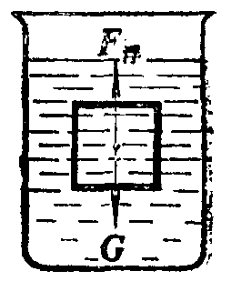
\includegraphics[width=3cm]{../pic/czwl1-ch6-6}
    \caption{物体在液体中受到浮力和重力}\label{fig:6-6}
    \end{minipage}
    \qquad
    \begin{minipage}{7cm}
    \centering
    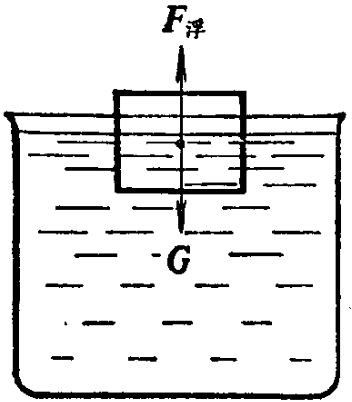
\includegraphics[width=4cm]{../pic/czwl1-ch6-7}
    \caption{浮在液面上的物体受到的浮力等于物体受到的重力}\label{fig:6-7}
    \end{minipage}
\end{figure}

\textbf{浸没在液体中的物体,如果受到的浮力大于它受到的重力,物体就上浮;
如果浮力小于重力,物体就下沉;
如果浮力等于重力,物体就可以停留在液体里任何深度的地方}。

木决完全浸没在水里的时候,因为木料的密度小于水的密度,所以木块比同体积的水轻,
也就是说,木块受到的浮力比木块受到的重力大,所以木块上浮。
露出水面以后,木块再继续上浮时,排开的水就逐渐减少,浮力也随着减小,
直到浮力减小到跟木块重相等时,浮力和重力互相平衡,木块就不再上浮。
因此,\textbf{漂浮在液面上的物体受到的浮力等于物体受到的重力}(图 \ref{fig:6-7})。


铁块浸没在水里的时候,因为铁的密度比水的密度大,所以铁块比同体积的水重,
也就是说,铁块受到的浮力小于铁块受到的重力,所以铁块下沉。
把一块铅皮揉成团放在水里,由于铅的密度比水的密度大,以铅团在水里也下沉(图 \ref{fig:6-8} 甲)。
\begin{figure}[htbp]
    \centering
    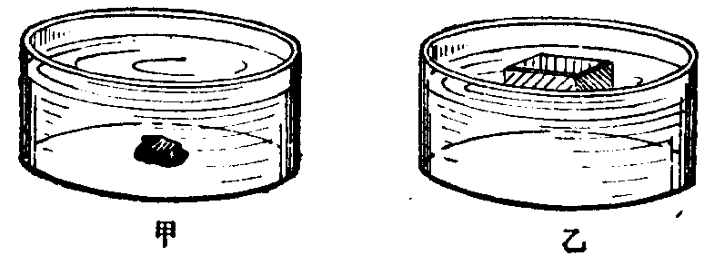
\includegraphics[width=0.6\textwidth]{../pic/czwl1-ch6-8}
    \caption{铅团下沉,铅盒浮在水面上}\label{fig:6-8}
\end{figure}
如果把铅皮做成盒子,铅皮受到的重力虽然没有改变,但是空心的铅盒的体积比铅团的体积大得多,
排开的水也就多,因此受到的浮力就大,所以铅盒能够浮在水面上(图 \ref{fig:6-8} 乙)。

由此可见,如果要用密度大于水的材料制成能够浮在水面的物体,可以把它做成空心的,使它能够排开更多的水。
人们就是根据这个道理,用密度大于水的钢铁制造了轮船、舰艇。

轮船的大小通常是用轮船的排水量表示的。轮船的排水量就是轮船装满货物后排开的水重。
轮船在安全所允许的情况下,满载货物时,水表面和船舷相交的线叫做载重线,
一般把它画在船壳外表面上。装货时不能使载重线的上缘没入水面以下,否则会发生危险。


\liti 有一个空心铝球,重 4.5 牛顿,体积为 $0.5\lffm$,如果把这个铝球浸没在水中,
它受到的浮力是多大?它是上浮还是下沉?

解:铝球受到的浮力
$$ F_\text{浮} = G_\text{水} = \rho_\text{水} gV_\text{排} = 1000 \qkmlfm \times 9.8 \ndmqk \times 0.0\; 005\lfm = 4.9 \niudun \;\juhao$$

$4.9 \niudun > 4.5 \niudun$,浮力大于重力。

答:铝球受到的浮力是 4.9 牛顿,把它浸没在水中它将上浮。


\lianxi

(1) 冰块为什么浮在水面上?

(2) 为什么铁块在水中下沉,而在水银中却能浮在液面上?

(3) 船从河里开到海里的时候,是沉下去一些还是浮起来一些?为什么?

(4) 水雷重 4400 牛顿,体是 $500\lffm$。把它浸没在水中,受到的浮力是多大?水雷是浮在水面还是沉入水底?



